\documentclass[border={0.1cm 0.1cm 0.1cm 0.1cm}]{standalone}  %E,S,W,N

\usepackage{amssymb}
\usepackage{amsmath}
\usepackage{tikz}
\usetikzlibrary{calc}	%for centerarc

\def\centerarc[#1](#2)(#3:#4:#5) {\draw[#1] ($(#2)+({#5*cos(#3)},{#5*sin(#3)})$) arc (#3:#4:#5);}

\begin{document}
	
	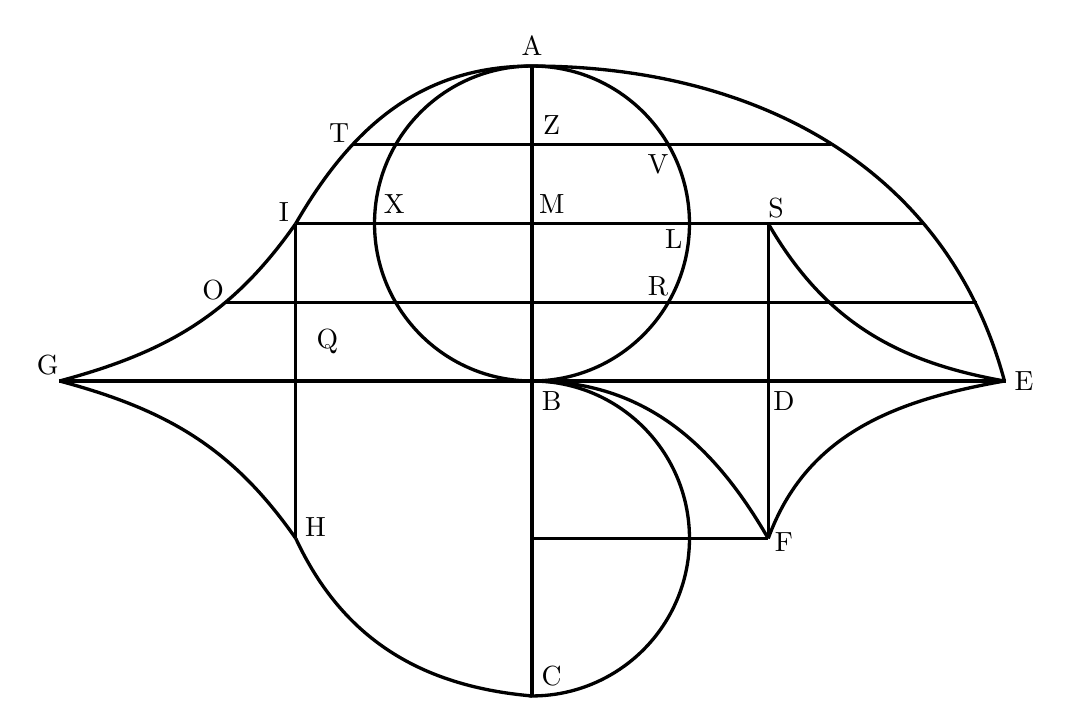
\begin{tikzpicture}[very thick]
	%LINES 
	\draw (0,-4)--(0,4); %vertical
	\draw (-3,2)--(-3,-2);
	\draw ( 3,2)--( 3,-2);
	%
	\draw (-6.01,0)--(6.0185,0); %horizontal
	\draw (-3.9,1)--(5.65,1);
	\draw (-3,2)--(4.98,2);
	\draw (-2.28,3)--(3.8,3);
	\draw (0,-2)--(3,-2);
	
	%UPPER PART
	\draw (0,2) circle (2cm);
	\centerarc[](0,3.25)(-22.5:-157.5:3.25cm)
	\centerarc[](0,0.75)(22.5:90:3.25cm)
	\draw (0,4) to[out=0,in=105] (6,0);
	\draw (3,2) to[out=300,in=170] (6,0);
	\draw (0,4) to[out=180,in=60] (-3,2);
	\draw (-3,2) to[out=235,in=15] (-6,0);
	
	%LOWER PART
	\centerarc[](0,-0.75)(-22.5:-90:3.25cm)
	\draw (0,0) to[out=0,in=120] (3,-2);
	\draw (0,0) arc (90:-91:2cm);
	\draw (3,-2) to[out=70,in=190] (6,0);
	\draw (0,-4) to[out=-185,in=-65] (-3,-2);
	\draw (-3,-2) to[out=-235,in=-15] (-6,0);
	
	%LABELS
	\node at (0.25,-0.25) {B};
	\node at (0.25,2.25) {M};
	\node at (0.25,3.25) {Z};
	\node at (1.6,2.75) {V};
	\node at (1.8,1.8) {L};
	\node at (1.6,1.2) {R};
	\node at (0,4.25) {A};
	\node at (-1.75,2.25) {X};
	\node at (-2.45,3.15) {T};
	\node at (-3.15,2.15) {I};
	\node at (-4.05,1.15) {O};
	\node at (-6.15,0.2) {G};
	\node at (-2.6,0.5) {Q};
	\node at (-2.75,-1.85) {H};
	\node at (0.25,-3.75) {C};
	\node at (3.2,-2.05) {F};
	\node at (3.2,-0.25) {D};
	\node at (3.1,2.2) {S};
	\node at (6.25,0) {E};
	\end{tikzpicture}
	
\end{document}